%!TEX root=main.tex
 % \vspace{-10pt}
 \section{Introduction\label{sec:intro}}
 % one for each key finding: a) many features deemed to be of importance to VQSs by domain experts, not all supported by present-day VQSs b) sketch is inefficient, perhaps explaining why present-day VQSs are not popular c) identify 3 typical workflows involving various sensemaking modalities in different proportions, depending on the application
 %To discover patterns of interest, analysts construct line chart visualizations \cut{using toolkits like \texttt{ggplot} or \texttt{matplotlib}, or visualization construction interfaces like Excel or Tableau,} \change{by} specifying {\em exactly} what they want to visualize. For example, when trying to find celestial objects corresponding to supernovae, which have a specific pattern of brightness over time, astronomers individually inspect the corresponding line chart for each object---numbering in the hundreds---until they find ones that match the pattern.
 Line charts are commonly employed during data exploration---the intuitive connected patterns often illustrate complex underlying processes
 and yield interpretable and visually compelling data-driven narratives~\cite{Few2012}. 
%To discover patterns of interest, analysts often have to construct and inspect thousands of line chart visualizations manually to find ones that match their desired pattern.
 However, discovering line charts that display certain meaningful patterns, trends, or characteristics of interest is often  an overwhelming and error-prone process, consisting of manual examination of large numbers of line charts. For example, when trying to find supernovae, which exhibits a unique pattern of brightness over time (an initial peak followed by a long-tail decay), astronomers often have to manually construct and inspect thousands of line chart visualizations to find ones with their desired pattern.
 %\techreport{For example, when trying to find celestial objects corresponding to supernovae, which have a specific pattern of brightness over time, astronomers individually inspect the corresponding line chart for each object---numbering in the hundreds---until they find ones that match the pattern.}\ccut{Similarly, when trying to infer relationships between two physical properties for different subsets of battery electrolytes, scientists need to individually visualize these properties for each subset (out of an unbounded number of such subsets) until they identify relationships that make sense to them.} 
 %This process of manual exploration of large numbers of line charts \change{for pattern identification} is not only error-prone, but also overwhelming for analysts. 
 To address this exploration challenge, there has been a large number of papers dedicated to building \emph{Visual Query Systems} (VQSs)---a term coined by Ryall et al.~\cite{ryall2005querylines} to describe systems that allow users to specify and search for desired line chart patterns via visual interfaces~\cite{mohebbi2011google,Hochheiser2004,wattenberg2001sketching,Siddiqui2017VLDB,ryall2005querylines,correll2016semantics,Mannino2018,Eichmann2015,Holz2009}. %visual patterns via interactive 
 These interfaces typically include a sketching canvas where users can draw a visual pattern of interest, with the system automatically traversing all potential visualization candidates to find those that match the specification. 
 % \par While this intuitive specification interface appears to be a promising solution
 \par While these intuitive specification interfaces were proposed as a promising solution to the problem of painful manual exploration of visualizations for time-series analysis~\cite{ryall2005querylines,wattenberg2001sketching}, to the best of our knowledge, VQSs have not lived up to these expectations and are not very commonly used in practice. One likely reason for the lack of VQS adoption may be attributed to how prior work \rchange{has} focused almost exclusively on optimizing the pattern-matching algorithms and interactions, with few invested in understanding actual user needs and how VQSs can be used for solving real-world problems. {\em Our paper seeks to understand how VQSs can actually be used in practice, as a first step towards the broad adoption of VQSs in data analysis}. Unlike prior work on VQSs, we set out to not only evaluate VQSs in-situ on real problem domains, but also involve participants from these domains in the VQS design. We present findings from a series of interviews, contextual \rchange{inquiry}, participatory design, and user studies with scientists from three different domains---{\em astronomy, genetics,} and {\em material science}---over the course of
 a year-long collaboration. The amount of time we invested in each of these three diverse domains surpasses the norm in this field and is key to uncovering the insights presented in this paper. As illustrated in Figure~\ref{science_goal}, these domains were selected to capture a diverse set of goals and datasets wherein VQSs can help address important scientific questions, such as: How does a treatment affect the expression of a gene in a breast cancer cell-line? Which battery components have sustainable levels of energy-efficiency and are safe and
 cheap to manufacture in production?
 \begin{figure}[ht!]
 	\centering
 	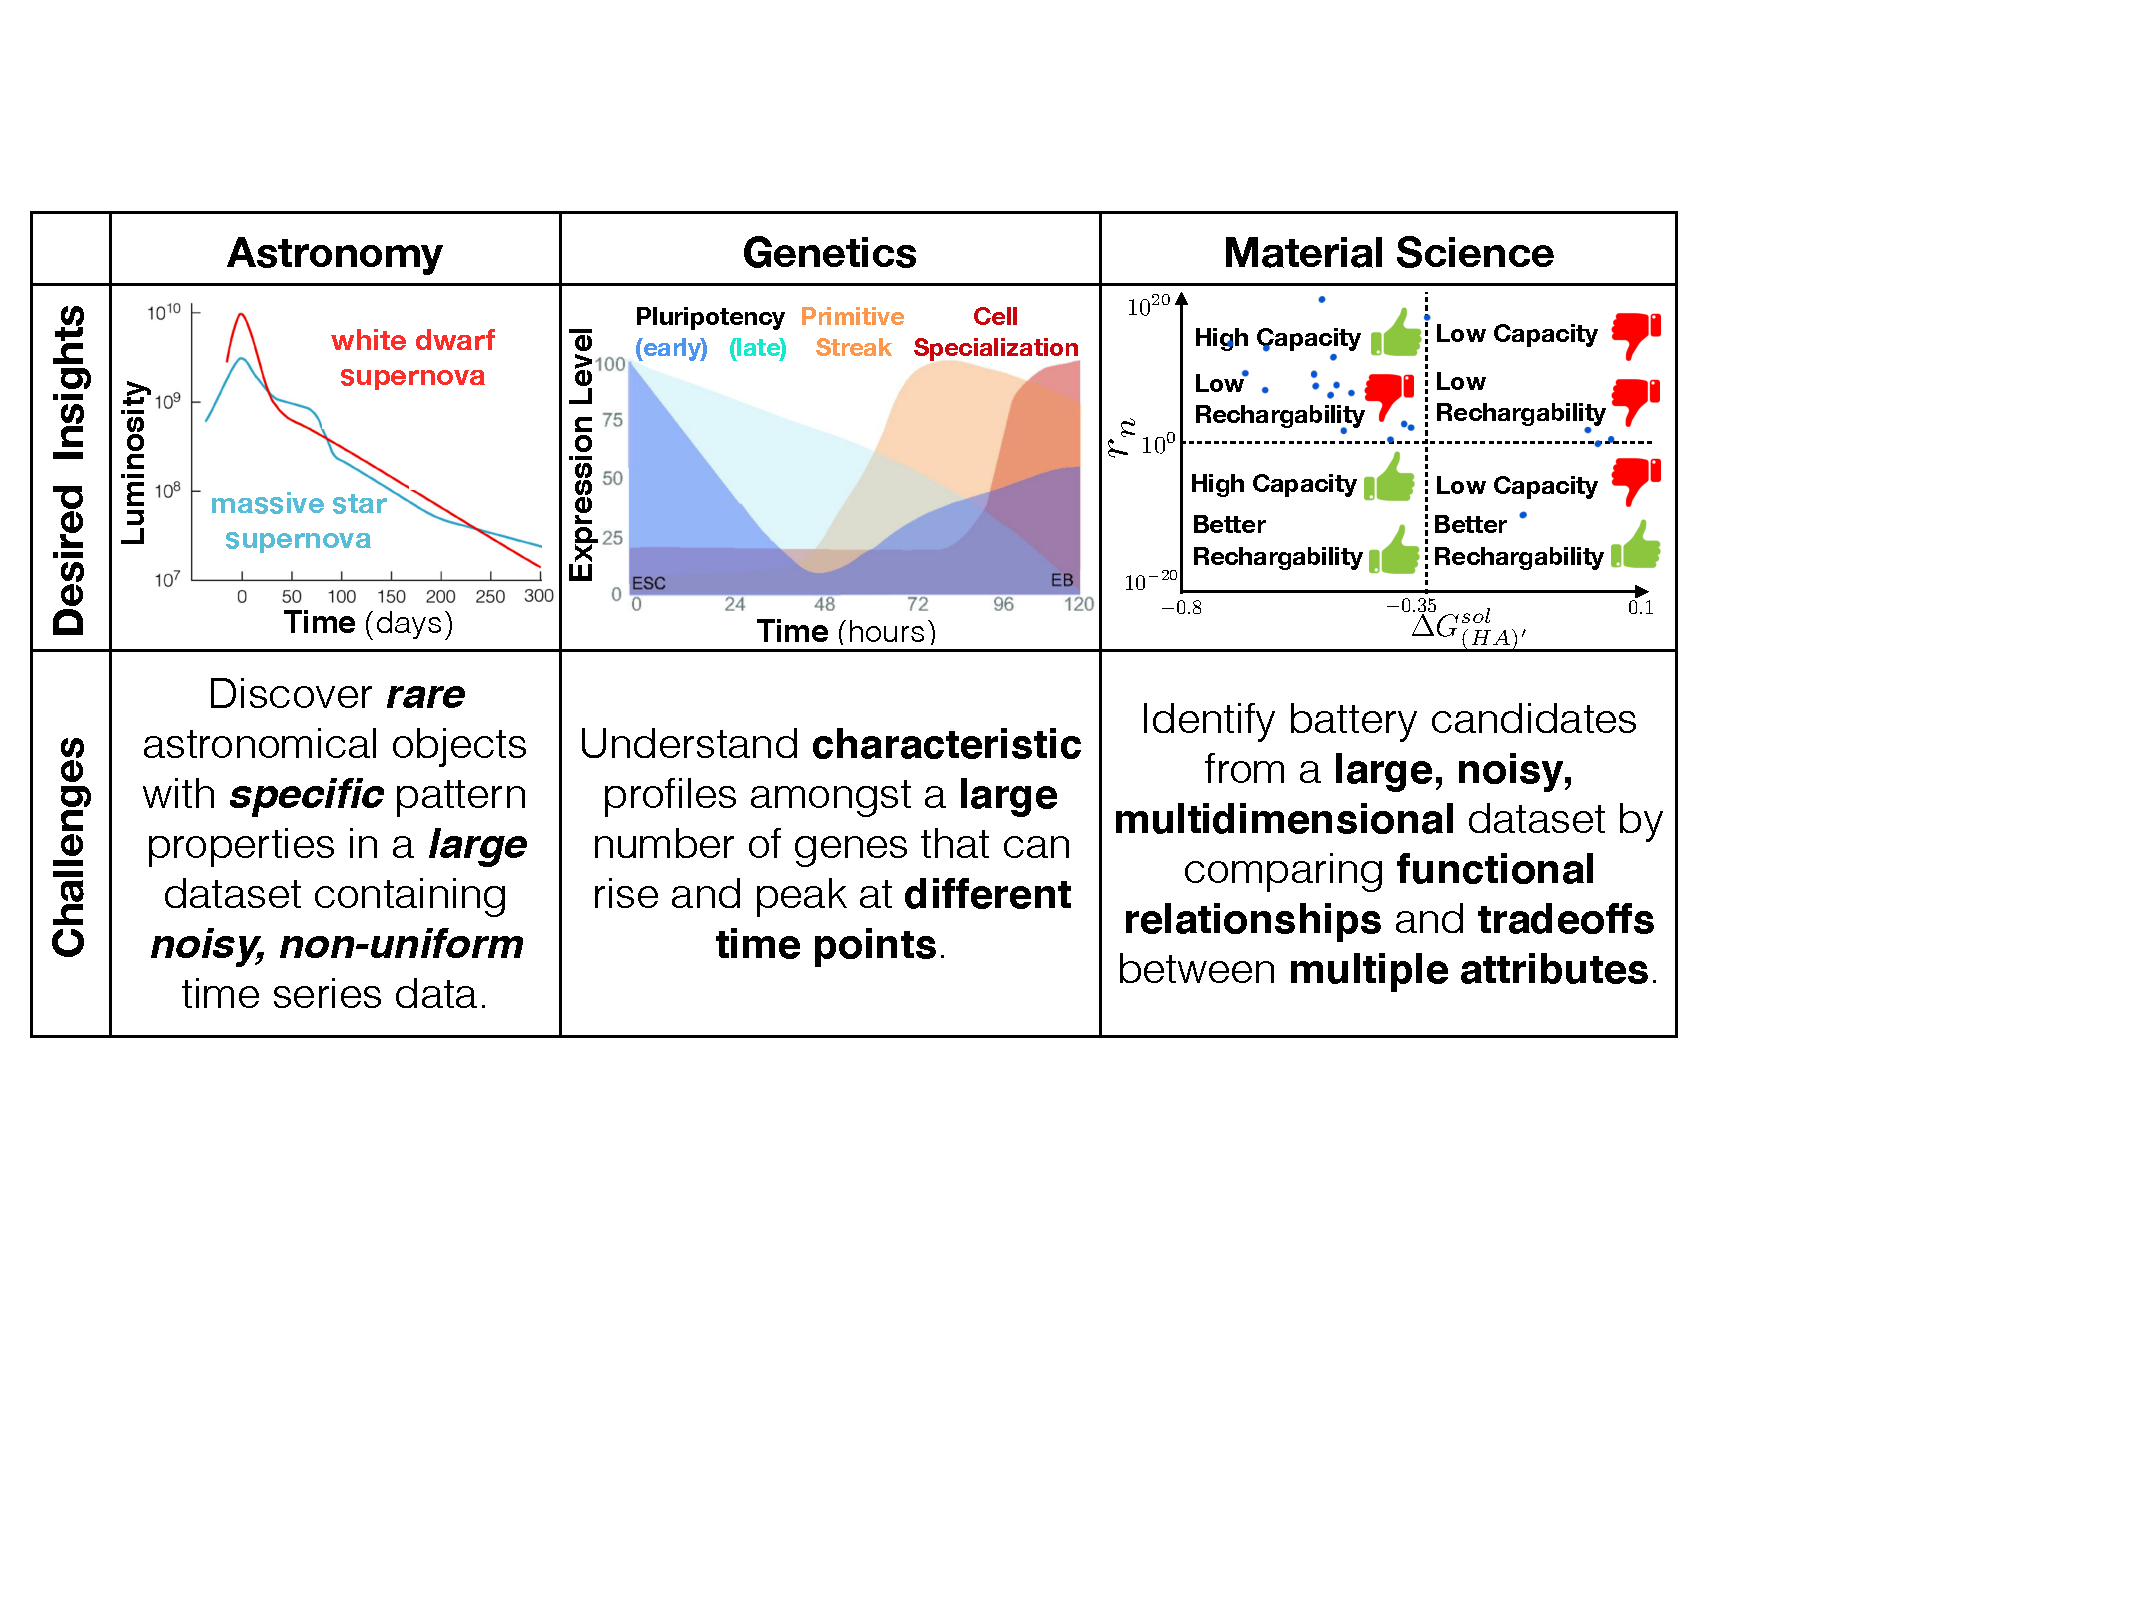
\includegraphics[width=\linewidth]{figures/science_goal.pdf}
 	\caption{Desired insights, problem and dataset challenges for each of the three application domains in our study.}
 	\label{science_goal}
 	\vspace*{-15pt}
 \end{figure}
 %\rchange{adopted a user-centered design approach to engage}
 \par Via contextual \rchange{inquiry} and interviews, we first identified challenges in existing data analysis workflows in these domains that could be potentially addressed by a VQS. Building on top of an existing open-source VQS, \zv~\cite{Siddiqui2017,Siddiqui2017VLDB}, we engaged participants in a process of \rchange{user-centered design~\cite{Norman1986,Nielsen1994} with participatory design elements~\cite{Muller1993,Schuler1993}} to enable them to better compose data exploration workflows that lead to insight discovery, over the course of a year. Rather than targeting a domain-specific solution, we \rchange{engaged with} multiple domains (an uncommon practice in visualization design studies) to observe differences and commonalities across domains and synthesize high-level insights regarding the use of VQSs. While designing and performing this multi-phased, mixed-methods research agenda across three diverse use cases was challenging, this endeavor was necessary for addressing the qualitative, participant-centered research questions investigated.%\dor{Aditya suggested changing participant-centered to user-adoption-centric, but participant-centered is a more commonly-used term.}}
 \par We organize our \cut{PD}\rchange{design study} findings into a taxonomy of VQS capabilities, involving three sensemaking processes inspired by Pirolli and Card's notional model of analyst sensemaking~\cite{Pirolli}. The sensemaking processes include \emph{top-down pattern search} (translating a pattern ``in-the-head'' into a visual query), \emph{bottom-up data-driven inquiries} (querying or recommending based on data), and \emph{context-creation} (navigating across different collections of visualizations). We find that prior VQSs have focused on enabling top-down processes (via sketching capabilities), but have largely overlooked the two other processes that we found to be essential in all three domains. These missing capabilities partially \rchange{explain} why prior VQSs have not been widely adopted in practice.
% other two processes that we found to be crucial for all three domains.
 %to gather feedback and iterate on VQS feature designs, culminating in a new enhanced VQS, \zvpp.
 \par To study how various VQSs are used in practice, we conducted a final evaluation study with nine participants using our final VQS prototype to address their research questions on their own datasets. During this 1.5-hour study, participants gained novel scientific insights,
 such as identifying a star that was known to harbor a Jupiter-sized planet, discovering a previously-unknown relationship between solvent properties, and finding characteristic gene expression profiles confirming the results of a related publication. %\techreport{Participants also gain additional insights about their datasets, including debugging mislabeled features and uncovering erroneous data preprocessing procedure applied to a collaborator's dataset.}%\techreport{, and discovering that the dip in an astronomical light curve is caused by saturated imaging equipment overlooked by the existing error-detection pipeline.}
 %\agp{Explain why these findings are important.}\dor{I think saying that planetary discovery is related to future colonization is a bit too much here and significance of characteristic gene expression profiles. Also we already described the significance of each domain earlier with the `important scientific questions' part.}
 %that goes from a pattern in-the-head to a desired visualization
 \par \rchange{During the evaluation study}, we were somewhat surprised to discover that sketching a pattern for querying is often ineffective on its own. This is due to the fact that sketching makes the \cut{problematic} assumption that users know the pattern that they want to sketch and are able to sketch it precisely. However, this is not the case in practice. For example, the geneticists from our study often did not have a preconceived knowledge of what to sketch for and relied heavily on VQS-recommended common and outlying patterns to jumpstart their queries. Likewise, while the material scientists from our study were interested in datapoints that fall within specific value-ranges, they did not have an apriori notion of what their desired patterns would look like. Overall, participants typically opted to combine sketching with other means of pattern specification---one common mechanism was to drag-and-drop a recommended pattern onto the canvas, and then modify it (e.g., by smoothing it out). %\cut{However, most VQSs do not support these other mechanisms (as we argued earlier, they typically focus only on top-down sensemaking processes, without covering bottom-up and context creation)}\dor{cutting this out since already mentioned 2 paragraphs ago}.
 %Participants were, however, able to apply the two other sensemaking processes to gain novel scientific insights, such as identifying a star with a transient pattern that was known to harbor a Jupiter-sized planet, finding characteristic gene expression profiles confirming the results of a related publication, and discovering mislabelled features from a data preprocessing mistake.
 % Further analysis of how participants transition between different sensemaking processes during analysis using a Markov model illustrated
 \par To further understand how participants engaged with VQSs in their analytical workflows, we constructed a Markov model to characterize how participants transitioned between different sensemaking processes during their analysis. We found that participants often constructed a diverse set of analytical workflows tailored to their domains by focusing around a primary sensemaking process, while iteratively interleaving their analysis with the two other processes. This finding points to how all three sensemaking processes, along with seamless transitions between them, are crucial for enabling the effective use and adoption of VQSs for addressing real-world challenges.%for data exploration.%For example, participants often center on a main sensemaking process, while interleaving variations with other two processes as they iterate on an analytic task.
 %---including the construction of a Markov model---
 \par To the best of our knowledge, our study is the \emph{first to holistically examine how VQSs can be designed to fit the needs of real-world analysts, and how they are actually used in practice}. Working with participants from multiple domains enabled us to compare the differences and commonalities across different domains, thereby identifying general VQS challenges and requirements for supporting common analytical goals. Our contributions include:
 \begin{denselist}
 \item a characterization of the problems addressable by VQSs through design studies with three different domains,
 \item a taxonomy of essential VQSs capabilities, leading to a sensemaking model for VQSs\cut{, grounded in participatory design findings}, %, as well as an articulation of the problem space that is amenable to VQSs %the construction of 
 \item an integrative VQS, \zvpp\cut{, post participatory design,} capable of facilitating rapid hypothesis generation and insight discovery, \rchange{resulting from iteration with end-users}, 
 \item study findings on how VQSs are used in practice, leading to the development of a novel sensemaking model for VQSs. %including the ineffectiveness of
 %evaluation
 % sketching and the ---- workflow
 \end{denselist}
 Our work not only opens up a new space of opportunities beyond the narrow use cases considered by prior studies, but also advocates common design guidelines and end-user considerations for building next-generation VQSs.